\documentclass{standalone}
\usepackage{graphicx}	
\usepackage{amssymb, amsmath}
\usepackage{color}

\usepackage{tikz}
\usetikzlibrary{shapes}
\usepackage{pgfmath}

\definecolor{light}{RGB}{220, 188, 188}
\definecolor{mid}{RGB}{185, 124, 124}
\definecolor{dark}{RGB}{143, 39, 39}
\definecolor{highlight}{RGB}{180, 31, 180}
\definecolor{gray10}{gray}{0.1}
\definecolor{gray20}{gray}{0.2}
\definecolor{gray30}{gray}{0.3}
\definecolor{gray40}{gray}{0.4}
\definecolor{gray60}{gray}{0.6}
\definecolor{gray70}{gray}{0.7}
\definecolor{gray80}{gray}{0.8}
\definecolor{gray90}{gray}{0.9}
\definecolor{gray95}{gray}{0.95}

\newcommand*{\offset}{0.025}

\begin{document}

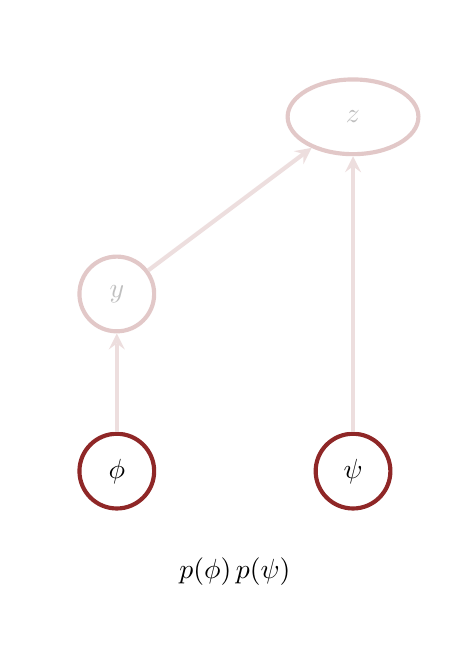
\begin{tikzpicture}[
   scale=0.2,
   obscirc/.style={circle, draw=dark, fill=dark, line width=1.5, text=white,
               inner sep=5, minimum size=27},
   obsell/.style={ellipse, draw=dark, fill=dark, line width=1.5, text=white,
                  inner sep=5, minimum height=27},
   unobscirc/.style={circle, draw=dark, fill=white, line width=1.5, text=black,
                     inner sep=5, minimum size=27},
   unobsell/.style={ellipse, draw=dark, fill=white, line width=1.5, text=black,
                    inner sep=5, minimum height=27}
  ]

  % Node Spacing
  \pgfmathsetmacro{\d}{7.5}
  
  \begin{scope}[shift={(0, 0)}]
    \draw[white] (-1.75 * \d, -1.25 * \d) rectangle (1.75 * \d, 3.75 * \d);
  
    \node (A) at (-\d, 0) [unobscirc] { $\phi$ };
    \node (B) at (+\d, 0) [unobscirc] { $\psi$ };
    
    \node (C) at (-\d, 1.5 * \d) [unobscirc] { $y$ };

    \node (D) at (+\d, 3 * \d) [unobsell] { $\hphantom{z = 1}$ };
    \node at     (+\d, 3 * \d) { $z$ };

    \foreach \B/\E in {A/C, B/D, C/D} {
      \draw[->, >=stealth, color=mid, line width=1.5] (\B) -- (\E);
    }
    
    \fill[white, opacity=0.75] (+1.75 * \d, +0.334 * \d) rectangle (-1.75 * \d, +3.5 * \d);
    
    \node at (0, -0.85 * \d) { $p(\phi) \, p(\psi)$ };

  \end{scope}

\end{tikzpicture}

\end{document}  